\chapter{Pixels detectors for the new ATLAS Inner Tracker}
\label{chap:ITk}

In this Chapter the new ATLAS Inner Tracker (ITk) of the ATLAS detector will be discussed. It is intended to be ready 
for  the data taking in 2026, in time for the beginning of the High Luminosity phase of the LHC (HL-LHC). 
The plans for the upgrades of the LHC are presented in Section~\ref{sec:HL-LHC}, along with the 
physics case and the list of ATLAS sub detector upgrades for the Phase-II; 
Section~\ref{sec:NewTracker} will cover the performance and specifications for the new ATLAS ITk. 
After describing the R\&D efforts for ITk pixels detectors in general (Section~\ref{sec:ITkPixels}), 
in Section~\ref{sec:radhardpixels} results for radiation hard pixel sensors will be presented. 
The concept of slim edge, already applied to IBL pixel sensors (Section~\ref{sec:IBLoverview}) will be 
pushed to its limits for the ITk pixels sensors; this topic will be discussed in details in 
Section~\ref{sec:edgeless}, together with results from beam tests. 
Finally conclusions and perspectives will be drawn in Section~\ref{sec:itksummary}.



\section{High Luminosity LHC and the Phase-II of the LHC experiments}
\label{sec:HL-LHC}

The timeline of the CERN LHC is presented in Figure~\ref{fig:HL-LHC-plan-2016-01}, together 
with the future plans. The High Luminosity LHC (HL-LHC)~\cite{HL_LHC} is a project, recently 
approved~\cite{HL-LHCApproval},  to upgrade the existing LHC to a high luminosity machine, 
capable to deliver an instantaneous luminosity of $L=7.5\times10^{34}$/cm$^{2}$/s; as a 
reminder the design luminosity of LHC is of $L=1.0\times10^{34}$/cm$^{2}$/s.
\begin{figure}[!htpb]
\centering
\includegraphics[width=1.0\textwidth]{HL-LHC-plan-2016-01.png}
\caption{\label{fig:HL-LHC-plan-2016-01}LHC/ HL-LHC Plan (last update 22.02.2016, after~\cite{HL_LHC})}
\end{figure}
After the HL-LHC upgrade completion the data taking  is expected to restart in 2026; the goal 
is to integrate a dataset of 3000~\invfb by 2037; there is an option to extend this program to arrive 
at 4000~\invfb.

As it can be seen in Figure~\ref{fig:HL-LHC-plan-2016-01} the upgrade plans don't include any increase 
of the center-of-mass energy $\sqrt{s}$. Thus, the main motivation for the HL-LHC project is 
reducing the error halving time. Indeed, taking data beyond 2023 at the same instantaneous luminosity of 
Run~3 would imply  to take data for more than 15 years to reduce the statistical error by a factor of 2.

The large dataset at the end of the so-called Phase 2 (or {\it} Phase-II) for the experiments should enable 
a  large program of precision measurements of the Higgs boson and New Physics (NP) discoveries. 
As an example of the potential of the HL-LHC dataset, the projected precision on coupling of the Higgs
 boson to $\mu$s is of about 7\% with  3000~\invfb; the Higgs 
trilinear self coupling parameter $\lambda_{HHH}$ can be probed at about 1 $\sigma$ significance 
in the range $-0.8<\lambda_{HHH}/\lambda_{SM}<7.7$ ($\lambda_{SM}$ is the SM predicted value) 
in the final state $HH\to\b\bbar\gamma\gamma$~\cite{ATL-PHYS-PUB-2014-016}. 
For what concerns NP potential discoveries, as an example, with the expected HL-LHC dataset the 
supersymmetric\footnote{Supersymmetry (SUSY) is a proposed type of spacetime symmetry where  each 
SM particle is associated with another particle, known as its superpartner, the spin of which differs by a 
half-integer; for an introduction to SUSY see~\cite{SusyPrimer}} top quark partner $\widetilde{t}$, 
the {\it stop}, discovery mass range extends up to 480~GeV, and the exclusion one to 700~GeV~\cite{ATL-PHYS-PUB-2016-022};
for the electroweak SUSY particles a factor of ten increase in luminosity translates into a 30-40\% increase in mass reach. Other than SUSY the physics program 
during the Phase-II of the LHC experiments include searches of   vector bosons resonances like 
$W',Z'$, 
extra dimensions and more~\cite{ATLASLoIPhaseII}.

The high luminosity foreseen for the Phase-II implies a much harsher environment than in Run~2 
for the ATLAS sub-detectors; indeed high luminosity means higher event rate, more pileup events 
and higher radiation doses and fluences. 
To cope with the severe data taking conditions expected at the HL-LHC it is planned to 
upgrade the  ATLAS detector~\cite{ATLASLoIPhaseII,ATLASITkScopingDocument}. Upgrades include:

\begin{itemize}
\item a longer latency trigger system, to cope with higher event rates,
\item new inner muon barrel trigger chambers, to assure redundancy and improve efficiency,
\item upgrading the tile calorimeter electronics, since the actual system will not survive the doses expected by the time of HL-LHC and
\item a complete new silicon only tracker, with coverage down to pseudorapidity $|\eta|=4$, the {\it Inner Tracker} (ITk)
\end{itemize} 

The constraints, requirements, layout and expected performance of the proposed ATLAS ITk will 
be discussed in the next Section.

\section{The Quest for a New ATLAS Inner Tracker}
\label{sec:NewTracker}

The new ATLAS  Inner Tracker will have to face unprecedented levels of radiation doses and fluences, 
pileup events and events rate. Table~\ref{tab:ITkConditions} summarises some of the most important figures.

\begin{table}[!htpb]
\centering
\caption{\label{tab:ITkConditions}Environment conditions for the inner detector at the LHC and HL-LHC}
\begin{tabular}{lcc}
\hline
\hline
Parameter & LHC & HL-LHC \\
\hline
instantaneous luminosity $L$	 [cm$^{-2}$s$^{-1}$] & $1.0\times10^{34}$ &  $7.5\times10^{34}$ \\
number of pileup events $\mu$ & 25 & 200\\
track rate density for the innermost pixel layer $\mathcal{N}$ [MHz~cm$^{-2}$] & 0.25 & 2 \\ 
fluence to the innermost pixel layer $\Phi$ [ 1 MeV $n_\text{eq}/\text{cm}^2$] & 5$\times10^{15}$ & 2$\times10^{16}$ \\
total ionising dose to the innermost pixel layer TID [MRad] & 160  & 1700 \\
\hline
\end{tabular}
\end{table}

Within this hostile environment the ITk will have to guarantee the same level of performance  or better 
of the ATLAS Inner Detector (ID).
The project is presented  in a series of documents, from the ``Letter of Intent for the Phase-II Upgrade of the ATLAS Experiment''~\cite{ATLASLoIPhaseII} to the ``ATLAS Phase-II Upgrade Scoping Document''~\cite{ATLASITkScopingDocument}. Technical Design Report (TDR) for strip detector of the 
ITk was recently published~\cite{ITkStripsTDR}; the ITk pixel detector TDR is due by the end of 2017.
This Section is built on those documents.




\subsection{Performance Requirements of the ITk}
In what follows a short list of performance requirements of the ITk.

\paragraph{Track Reconstruction Efficiency}
The required 
track reconstruction efficiency in the central part ($|\eta|<2.7$) has to be above 99\% for muons with 
$p_T$ above 3~GeV/c, above 85\% for pions (electrons) with 
$p_T$ above 1(5)~GeV/c.  Fake tracks rate has to be kept below 1\% to avoid degrading resolution of 
objects built using tracks, like tracks jets.

\paragraph{Track Resolution and Vertex Reconstrucion}
The resolution on transverse momentum will be better than 0.5\% up $|\eta|=1$ for muons of 100~GeV/c 
$p_T$ and will degrade moderately till $|\eta|=2$. For $|\eta|\ge2.7$ the solenoid field diminishes, 
particularly at low radius, leading to poorer $p_T$ resolution. 
Resolution on longitudinal (transverse) parameter $d_0(z_0)$ are required to be better than 100~$\mu$m 
in the very central region $|\eta|<0.5$ for tracks with $p_T$~=~1GeV/c and better than 8 (50)~$\mu$m  
in the limit of very large transverse momentum.  
 
 With 200 pile-up events, the mean separation of primary vertices is typically less than 1~mm.
 It is therefore not possible for all vertices in a triggered event to be reconstructed individually. However, it is important that high transverse momentum objects (muons, electrons and tracks in high transverse energy jets) coming from a common vertex can all be correctly associated to the same vertex with good efficiency.
  This requirement corresponds, in the case of $\t\tbar$ events, to the probability of the $\t\tbar$  vertex being among the reconstructed vertices having to be greater than 0.95. In addition, the probability that the 
$\t\tbar$  decay is associated to the correct reconstructed vertex should be greater than 0.90.
 
 
 Tracking-reconstruction efficiency and minimisation of multiple scattering effects requirements impose a 
 low material budget. For the ITk, generally it is required to be in total <1 $\X_0$ up to $|\eta|\le2.7$.
 In Figure~\ref{fig:ITk_X0}.
  The ITk material budget is around 30\% lower in the region $|\eta|\le4.0$, compared to the Run~2 detector.
\begin{figure}[!htpb]
\centering
\includegraphics[width=0.49\textwidth]{ID_X0.png}
\includegraphics[width=0.49\textwidth]{ITk_X0.png}
\caption{\label{fig:ITk_X0}Material budget expressed as fraction of radiation lengths as a function of the 
pseudorapidity. (left) ATLAS ID (right) ATLAS ITk. (After~\cite{ITkStripsTDR})}
\end{figure}
  
\subsection{ITk detector layout}

The ITk will be an all silicon tracker; the main reason for abandoning the TRT is the projected occupancy 
in its straw tubes, which is about 100\% at $L=5.0\times10^{34}$cm$^{-2}$s$^{-1}$. 
The ITk will consist of an inner detector made of pixel modules and an outer one made of strips. 
In the central region of the ITk Detector, sensors are arranged in cylinders around the beam axis, with (starting from inside) five pixel layers followed by two short-strip layers of paired stereo modules then two long-strip layers of paired stereo modules. The forward regions will be covered by six strip disks and a number of pixel rings leading to one or more hits depending on the ring layer and $\eta$ position. 
The ITk layout is presented in Figure~\ref{fig:ITk_Layout}. The new tracker will cover a pseudorapidity range down to $|\eta|=4$. 

\begin{figure}[!htpb]
\centering
\includegraphics[width=0.65\textwidth]{ITk_Layout.pdf}
\caption{\label{fig:ITk_Layout}Schematic layout of the ITk for the HL-LHC phase of ATLAS. Here only one quadrant and only active detector elements are shown. The horizontal axis is the axis along the beam line with zero being the interaction point. The vertical axis is the radius measured from the interaction point. The outer radius is set by the bore of the solenoid. (After~\cite{ITkStripsTDR})}
\end{figure}

The peculiarity of the chosen ITk baseline layout, the so called ``Inclined'' layout, is the presence of 
inclined sensors in the forward part of the barrel layers; the inlined sensor hangs from  long 
barrel staves.
   This allows the material transversed by particles at 
large  $\eta$ to be minimised and at the same time requires less silicon surface to cover the full  $\eta$  
range. In addition, these inclined sensors provide two or more hits in the first layer, providing redundancy for the local track finding close to the interaction point even at large pseudorapidity.
One possible  support design of the Inclined layout is called ALPINE; a detail of the ALPINE stave 
prototype is shown in Figure~\ref{fig:ALPINE}.
\begin{figure}[!htpb]
\centering
\includegraphics[height=0.25\textheight]{ALPINE.pdf}
\caption{\label{fig:ALPINE}ALPINE design for the inclined layout (After~\cite{ITkStripsTDR})}
\end{figure}
The sensor modules are located on the stave face closer to the interaction point so that incoming particles 
are detected by a pixel sensor before crossing the inactive material (local support structure, cooling tubes 
and electrical services).

\section{Pixels Detectors for ITK}
\label{sec:ITkPixels}

The innermost pixel barrel layer, Layer 0, of the ITk will be at about 40~mm; the Layer 1 at 85~mm. 
Layer 2, 3 and 4 will be placed respectively at 155, 213 and 271~mm from the beam axis. 
The expected fluences for the ITk are reported in Figure~\ref{fig:ITk_Fluence}.

\begin{figure}[!htpb]
\centering
\includegraphics[width=0.65\textwidth]{ITk_Fluence.png}
\caption{\label{fig:ITk_Fluence} The 1 MeV neutron equivalent fluence  for the ITk layout 
(After~\cite{ITkStripsTDR})}
\end{figure}

The maximum fluence predicted for the Layer 0 at the end of the Phase-II program is about 1.5-2$\times10^{16}$~n$_{\rm eq}$/cm$^2$; for the pixel end-cap the largest fluence will be  of about 
5$\times10^{15}$~n$_{\rm eq}$/cm$^2$, similar to what it is expected for the Layer 1 of the barrel section.

Pixels will have a smaller pitch than today ATLAS pixel and IBL detectors; this is mandatory to keep  the 
occupancy below 1\%, in order to assure a good two particle separation and limit dead time. 
The proposed ITk layouts are designed to meet this requirement, thus the pixel pitches 
are dictated by this constraint. 
Moreover physics and performance simulations indicated that   50~$\mu$m~$\times$~50~$\mu$m pitch 
pixels, or 25~$\mu$m~$\times$~100~$\mu$m are suited (the smaller pitch is to achieve better 
momentum resolution).
Small pixel cells imply also less leakage current fed into and small capacitance coupled to the front end 
electronics, hence less noise. 


The basic  unit of the ITk pixel detector is a module. The baseline module concept for the ITk pixel detector is the well proven hybrid pixel detector in which modules are composed of a sensor and the read-out chip (ROIC) bump bonded to each other on a pixel level. In addition other concepts are also investigated such as monolithic CMOS pixel detectors especially for the outer layers.





The choice of sensors depends mainly on the requirement that the detector has to withstand the integration of an expected dataset  of 3000\invfb.  This is particularly challenging for the innermost layer, which after the high-luminosity running is exposed, as it was said above, to an estimated fluence $\Phi$ of 1.5-2$\times10^{16}$~n$_{\rm eq}$/cm$^2$ for the innermost pixel layer. 

There will be two main types of modules: dual-modules (two chips bump bonded to a sensor, around 
4~$\times$~2~cm$^2$) for the the innermost layer to accommodate the limited space, quad- modules (four 
chips bump bonded to a sensor, around 4 $\times$~4~cm$^2$ for the outer layers and in the rings. 
The read-out chip is presently under development within the RD53 collaboration~\cite{RD53}, 
which will produce an RD53 prototype chip. Following this chip an ATLAS ITk pixel chip will be developed 
using the basic blocks designed by RD53 while integrating additional functionality to meet ATLAS 
specifications.

At this stage three possible sensor types are considered for the pixels modules:

\begin{itemize}
\item planar sensors, for an hybrid detector
\item 3D sensors, again for an hybrid detector,
\item monolithic CMOS sensors
\end{itemize}

\paragraph{3D sensors}
3D silicon detectors are candidates to be used for the inner most layer(s) of the barrel pixel system and 
some of the inner end-cap rings due to their excellent radiation hardness at low operational voltages and 
moderate temperatures with low power dissipation compared to planar sensors.
The 3D sensors will be produced on either 4" or 6" high resistivity $p-$type wafers. 
The total thickness of the sensors will be 200~$\mu$m, and and the active thickness\footnote{sensors can be realised in thin high resistivity wafers bonded to thick low resistivity ones; at the end of the fabrication process the latter can be lapped, completely or not. This approach is used to realise thin planar sensors too} will be between 
150 and 200~$\mu$m, with 150~$\mu$m being the baseline. 
The 3D sensors shall be produced by etching the $p-$ and $n-$columns from the same side (single side process). At the moment the pixel geometry will have a single readout column in the centre of the pixel (1E), surrounded by four ohmic columns. Figure~\ref{fig:3D_design} shows the proposed design of the pixel 
cell for the ITk 3D pixel modules. 

\begin{figure}[!htpb]
\centering
\includegraphics[width=0.55\textwidth]{3D_design.pdf}
\caption{\label{fig:3D_design} Design of 3D pixel cells with 50~$\mu$m~$\times$~50~$\mu$m  and 25~$\mu$m~$\times$~100~$\mu$m pitch pixels. (After~\cite{ITkStripsTDR})}
\end{figure}

The column diameter will be $\le$~8~$\mu$m, while the depth of the junction (ohmic) columns will be 
slightly shorter (longer) than the nominal  150~$\mu$m active thickness. Thus ohmic columns will 
be in contact with the sensor backside, while junction columns termination will be away from it, to 
avoid too early junction break down.

IBL-generation 3D pixel detectors coupled to FE-I4 pixel electronics have been found to have hit efficiencies 
in test beam measurements larger than 97\% at 170 V after irradiation to $\Phi$ of 
1.0$\times10^{16}$~n$_{\rm eq}$/cm$^2$ for normally incident minimum ionizing particles with a power 
dissipation of 15 mW/cm$^2$ at a temperature of -25$^{\circ}$~C~\cite{1748-0221-11-11-C11024}.

\paragraph{Planar sensors}
In this Paragraph only a short description of the planar sensors specification and performance 
for the ITk will be given as they will be discussed more in depth in the next two Sections. 
A new generation of planar pixel sensors are under development for the ATLAS ITk pixel system. The main 
differences with respect to the planar sensors implemented in the present detector are the different 
electrode arrangement ($n-in-p$ versus the traditional $n-in-n$) and the reduced thickness in the range of 
100-150~$\mu$m with respect to the 200~$\mu$m for the sensors used in IBL and 250~$\mu$m 
in the three outer ATLAS pixel layers. 

The $n-in-p$ technology allows for cost reduction given the single side processing and the reduced 
complexity in handling and testing. The guard ring structure is implemented on the front side, leaving the 
edges of the sensor at a potential close to the one of the backside. This arrangement potentially induces the 
risk of electrical sparks between the sensor periphery and the chip. Isolation techniques, like the deposition 
of a layer of Benzocyclobutene (BCB) on the sensor surface at wafer level or of parylene after module 
	assembly have been successfully employed to prevent this problem~\cite{Stefano,UNNO201372}.

\paragraph{Monolithic CMOS sensors}
Recent developments of CMOS pixel detectors, originally designed for charge collection in an epitaxial layer 
of 10-20~$\mu$m thickness, use new approaches to cope with the rate and radiation environment expected 
at the HL-LHC~\cite{PERIC2007876,1748-0221-11-02-C02045,HEMPEREK20158} 
based on the following enabling technology features:
HV add-ons that allow to use high depletion voltages; high resistivity wafers for large depletion depths; 
radiation hard processed with multiple nested wells to allow CMOS electronics em-bedded with sufficient 
shielding into the sensor substrate; and backside processing and
thinning for material minimisation and backside voltage application.

A typical CMOS sensor pixel cell with sensing substrate and a CMOS electronics layer
embedded in multiple cells is shown in Figure~\ref{fig:DMAPS}.

\begin{figure}[!htbp]
   \centering
   \includegraphics[width=0.65\textwidth]{DMAPS.pdf} 
   \caption{\label{fig:DMAPS}DMAPS schematic showing fully or partially depleted bulk, multiple nested wells for CMOS electronics and charge collection node. (After~\cite{ITkStripsTDR})}
   \end{figure}

Since 2014 a demonstrator programme to prove DMAPS that are suited for high rate and high radiation 
operation at LHC. For this a number of technologies have been explored and characterised 
(AMS 350 nm and 180 nm, Global Foundry 130 nm, ESPROS 150 nm, LFoundry 130nm, TowerJazz 
180nm, etc.); the designs have been characterised as stand-alone sensors as well as bonded to the FE-I4 
pixel chip (as a ?hybrid?) either via bump bonds or via glue bonding (capacitively coupled pixel detector, 
CCPD).

The results within the demonstrator programme can be summarised as follows:
\begin{itemize}
\item Technologies complying with the above list of enabling technology are principally suited to fabricate depleted monolithic sensors that can cope with the HL-LHC running condition, at least at distances larger than 20-25~cm away from the interaction point (outer layers).
\item DMAPS pixel sensors detect mips with integrated efficiencies above 98\% 
and with spatial resolutions similar to those as hybrid pixels 
\item DMAPS pixel sensors can stand radiation fluences of more than 1.0$\times10^{15}$~n$_{\rm eq}$/cm$^2$ when properly designed. This is demonstrated in Figure~\ref{fig:Eff_DMAPS} showing the 
collection width obtained after irradiation to a neutron fluence of 8.0$\times10^{15}$~n$_{\rm eq}$/cm$^2$ 
determined using
edge TCT measurements~\cite{1748-0221-12-02-P02021,5402213}.
\item  Test beam measurements have shown high rate capability as detectors bonded to the FE-I4.
\item Fully monolithic DMAPS pixel sensors have been designed incorporating read-out architectures suitable to cope with the expected rates at the HL-LHC (such as column- drain architectures and direct hit transfer architectures). Such designs have been sub- mitted for fabrication in 2016 and are currently being evaluated.
\end{itemize}

\begin{figure}[!htbp]
   \centering
   \includegraphics[width=0.6\textwidth]{Eff_DMAPS.pdf}
   \caption{\label{fig:Eff_DMAPS}FWHM of the charge collection profile measures using the edge TCT 
   technique  as a function of bias voltage after 
   different irradiation fluences up to 8.0$\times10^{15}$~n$_{\rm eq}$/cm$^2$ for un-thinned detector 
   (700~$\mu$m thick) without back plane (full symbols) and 300~$\mu$m
    sample with back plane
(empty symbols). 
(After~\cite{1748-0221-12-02-P02021})}
\end{figure}

\section{Radiation Hard Planar Pixel Sensors}
\label{sec:radhardpixels}

The ATLAS Upgrade Planar Pixel Sensor (PPS) R\&D Project~\cite{PPS:proj} carried out the optimisation of the 
well-known technology of planar silicon pixel sensors for the Phase-II of the ATLAS experiment. 
The PPS R\&D project existed from 2009 to 2014 and investigated the radiation hardness of 
pixels sensors realised in planar technology. The main research directions were: optimisation 
of the $n-$bulk material; exploration of $p-$bulk sensors; reduction of thickness; novel biasing 
structures.  
Reduction of the dead are at the detector periphery was investigated too, but this will be discussed in the 
next Section. 
These efforts were then continued within the ITk forming collaboration. 

In what follows some results from the PPS activities.

\subsection{Radiation hardness of $n-in-n$ FE-I3 samples.}
In~\cite{BOMBEN2012940,1748-0221-7-10-P10028} examples of the searches within the PPS group 
are reported. Using pixel modules based on the ATLAS Pixel FE-I3 readout chip the charge collection 
efficiency (CCE) of $n-in-n$ modules was tested up to fluences 
$\Phi$=2.0$\times10^{16}$~n$_{\rm eq}$/cm$^2$. Table~\ref{tab:n-in-n} summarizes the fluences to which 
the sensors were irradiated.

\begin{table}[!htb]
\caption{\label{tab:n-in-n}Summary of irradiated n-in-n samples in the testbeams. KIT stands for 25\,MeV energy proton irradiation; reactor neutrons for the TRIGA reactor~\cite{SNOJ2011136}.
}
\begin{center}
\begin{tabular}{l|c|c|l}
name & thickness ($\mu$m)  & fluence ($10^{15}$\,n$_{\rm eq}$/cm$^2$) & irradiation type\\
\hline \hline
DO6 & 285 & 0 & -- \\
DO7 & 250 & 1 & protons (KIT)  \\
DO8 & 250 & 1 & reactor neutrons  \\
DO9 & 250 & 5 & reactor neutrons \\
DO10 & 250 & 20 & reactor neutrons \\
\hline
\end{tabular}
\end{center}
\end{table} 

These modules have been evaluated in several beam tests in 2009 and 2010.
Data presented in~\cite{1748-0221-7-10-P10028}  were taken in two different periods in 2010 at the CERN 
SPS beamline H6; in both periods pion beams of 120\,GeV/c were used.
Measurements on  samples have been carried out at temperatures well
below 0$^{\circ}$~C to reduce the large leakage current from irradiated
sensors. As an example, we measured a leakage current of 24~${\rm \mu A}$
 (10~${\rm \mu A}$) for DO10 (DO9), at a bias voltage of 1200~V and at
 -47$^{\circ}$~C.

\paragraph{Hit Efficiency}

Hit efficiency was studied as a function of the bias voltage, for the
module irradiated with $5\times 10^{15} n_{eq}/cm^{2}$.
Results are in table~\ref{tab:n-eff}.

\begin{table}[!htb]
\caption{\label{tab:n-eff}Hit efficiency of an irradiated (fluence = $5\times 10^{15} n_{eq}/cm^{2}$)
FEI3 $n-in-n$ 200~$\mu$m thick module at different bias voltages.}
\begin{center}
\begin{tabular}{|c|c|c|}
\hline
Bias voltage (V) & Hit efficiency (\%) \\
\hline
350 & 93.2 \\
\hline
500 & 97.3 \\
\hline
1000 & 99.6 \\
\hline
\end{tabular}
\end{center}

\end{table}

\begin{figure}[!htb]
\begin{center}
\includegraphics[width=0.49\textwidth]{5E15_onlyElectrons.png}
\includegraphics[width=0.44\textwidth]{EffMap_DO13_1000V.png}
\end{center}
\caption{\label{fig:5e15}left: Collected charge as a function of the bias for sensors irradiated
with fluence of $5\times 10^{15} n_{eq}/cm^{2}$; right: Hit efficiency map for the same assembly}
\end{figure}

In figure~\ref{fig:5e15}, on the left, a study of the collected charge vs bias voltage
 for a module irradiated with a fluence of $5\times 10^{15} n_{eq}/cm^{2}$ is shown\footnote{as
 a comparison data from~\cite{Casse} are reported too.} (only data collected with the
 $^{90}$Sr  source are shown).  In the figure the expected threshold for the FE-I4
 chip is shows too. A signal of about 10 ke$^-$ is observed at 1000 V. This was very
 promising for the  ATLAS IBL~\cite{IBLTDR}, and
  the outer pixel layers at HL-LHC.

In figure~\ref{fig:5e15}, on the right, the hit-efficiency map for the module irradiated with a
fluence of $5\times 10^{15} n_{eq}/cm^{2}$, as measured at the testbeam for particles
at normal incidence. The pixel module was biased at 1000 V and the hit-efficiency was 99.6\%.


\paragraph{Charge Collection Efficiency}
One of the main effects of irradiation is the increased trapping, which leads to a reduced signal amplitude. 
As the trapping probability depends on the charge carrier velocity, the collected charge was measured as a 
function of the bias voltage. Figure~\ref{fig:DO_all_Save} shows the results for all irradiated $n-in-n$ 
samples in the two beam test periods; see also Table~\ref{tab:n-in-n}. A systematic error on the collected 
charge of 400\,e is assumed, due to the finite charge resolution of the ToT mechanism;  a 5\% systematic 
uncertainty is also taken into account, due to non-uniformity in the injection capacitances.\\
After $5\times 10^{15}$\,n$_{\rm eq}$/cm$^2$, the collected charge still exceeds 10~ke at a bias voltage of 
1000\,V. Even if the collected charge is shared equally between two neighboring pixels, this charge is 
sufficient to detect the hit with FE-I3.

\begin{figure}[!htpb]
 \begin{center}
  \includegraphics[width=0.65\textwidth]{DO_all_Save.pdf}
 \end{center}
 \caption{\label{fig:DO_all_Save}Collected charge as a function of bias voltage for $n-in-n$ samples irradiated to different fluences
 (see details in the text).
 A threshold of 3200~e is indicated.}
\end{figure}

Figure \ref{fig:n-in-n:Oct_P5_D11_qeff} top, shows that charge is predominantly
 lost in the region of the punch-through bias grid system.

 At very high fluences ($2\times 10^{16}$\,n$_{\rm eq}$/cm$^2$, DO10 sample)
 it is no longer possible to say which region is less efficient than the others, using the charge collection method
 (Figure \ref{fig:n-in-n:Oct_P5_D11_qeff}, bottom).
\begin{figure}[!htb]
 \begin{center}
  \includegraphics[width=1\textwidth]{Oct_P8_1_9_9_1_D10_qeff.pdf}
  \includegraphics[width=1\textwidth]{Oct_P5_D11_qeff.pdf}
 \end{center}
 \caption{\label{fig:n-in-n:Oct_P5_D11_qeff}Charge collection within a pixel. Top: DO9 at V$_{bias}$=1200\,V. Bottom: DO10 at V$_{bias}$=1000\,V.}
\end{figure}

\paragraph{Charge Sharing Probability}

To calculate the charge sharing probability for each hit within a cluster, it is determined whether a hit is found in a pixel cell adjacent to the one matched to a track.
This probability increases towards the edge of the pixel since charge carriers are more likely to drift to the neighbouring pixel. The corresponding plot, referred to as a charge sharing map, is centred on one pixel, also showing half of the adjacent pixel in each direction.
The overall charge sharing is defined as the number of tracks with at least one hit in a neighbouring pixel divided by the number of all tracks.

Figure \ref{fig:n-in-n:DO9_qshare} shows the charge sharing probability for DO9 at a bias voltage of 1200\,V.
Reduced charge sharing probability is visible in the region of the bias dot
 and the bias grid network.\footnote{The bias grid network is an aluminum trace
 arranged on top of the intermediate pixel region connecting all bias dots.}
 Less charge is deposited here, so there is a higher probability for the second pixel in a two-pixel cluster to be below threshold.
As only the bias trace makes the difference between both pixel sides, it might cause the lower charge sharing probability. Furthermore, one can see that the region of the bias dot is not affected.

 While for DO9 a clear increase in charge sharing probability towards the edges of the pixel is visible, at higher fluence the collected charge becomes too small for any significant charge sharing to be observable. 
\begin{figure}[!htpb]
 \begin{center}
 \hspace{-.28cm}
  \includegraphics[width=0.887\textwidth]{n_pixel_charge_share_v5_2.png}
  \includegraphics[width=\textwidth]{Oct_P8_1_9_9_1_D10_qshare.pdf}
 \end{center}
 \caption{Top: Design of the sample of the region shown in the plot below. Bottom: Charge sharing probability for DO9 at V$_{bias}$=1200V. Note the reduced charge sharing in the bias grid region on the right-hand side of the central pixel. \label{fig:n-in-n:DO9_qshare}}
\end{figure}

\paragraph{Residuals}
To estimate the intrinsic spatial resolution of the devices under test (DUTs),
 the distribution of hit residuals was studied. The intrinsic spatial resolution was estimated by the RMS of the 
 residual distribution for clusters of all sizes, while the residual distribution of 2-pixel clusters is used to 
 estimate the width of the area between pixels, where charge sharing occurs. The distribution is fitted with 
 the sum of two Gaussian functions, where one accounts for misreconstructed hits, resulting in large 
 residual values (equal to 2 times the pixel pitch or more), and the other for correctly reconstructed hits. The 
 width of this ``core'' Gaussian gives the width of the charge sharing region.
 
 Figure \ref{fig:n-in-n:residuals} shows the residual distributions in the 50\,$\mu$m pixel direction for the unirradiated sample (DO6) and the sample irradiated to
\mbox{$2\times10^{16}\,{\rm n_{eq}}/{\rm cm}^2$}, respectively. The widths of the distributions are 16\,$\mu$m and 15.4\,$\mu$m, comparable with the expected digital resolution of 14.4\,$\mu$m. Thus, no influence of radiation damage on the spatial resolution can be observed.

\begin{figure}[!htb]
 \begin{center}
  \includegraphics[width=.49\textwidth]{Oct_Period1-residuals2-11-fitResY.pdf}
  \includegraphics[width=.49\textwidth]{Oct_Period5-residuals2-11-fitResY.pdf}
 \end{center}
 \caption{Residual distributions in the short pixel direction for an unirradiated sample (DO6, left) and a sample irradiated to $2\times 10^{16}$\,n$_{\rm eq}$/cm$^2$ operated at a bias voltage of 1000\,V (DO10, right). No deterioration of the spatial distribution with irradiation is visible. \label{fig:n-in-n:residuals}}
\end{figure}


Plotting the residual distribution for two-pixel clusters only allows the width of the charge sharing region between pixels to be determined. Figure \ref{fig:n-in-n:CS2-residuals} shows the distributions for DO9 ($5\times 10^{15}$\,n$_{\rm eq}$/cm$^2$) and DO10 ($2\times 10^{16}$\,n$_{\rm eq}$/cm$^2$). After correcting for the telescope resolution, the widths of the charge sharing regions are 7.1\,$\mu$m and 7.7\,$\mu$m. These values correspond very well with the width found for an unirradiated sample of 6.4\,$\mu$m. This indicates that the lateral diffusion of the charge cloud does not change significantly with irradiation.

\begin{figure}[!hbt]
 \begin{center}
  \includegraphics[width=.49\textwidth]{Oct_Period5_1-residuals2-10-cluSize2-multiG_resY.pdf}
  \includegraphics[width=.49\textwidth]{Oct_Period8_1-residuals2-11-cluSize2-multiG_resY.pdf}
 \end{center}
 \caption{Residual distributions for 2-pixel clusters only. Shown are distributions samples irradiated to $5\times 10^{15}$\,n$_{\rm eq}$/cm$^2$ (left: DO9, bias voltage 1000\,V) and $2\times 10^{16}$\,n$_{\rm eq}$/cm$^2$ (right, DO10, bias voltage 1200\,V), respectively. \label{fig:n-in-n:CS2-residuals}}
\end{figure}

\paragraph{Comments}
The radiation hardness of $n-$bulk sensors was tested up to unprecedented fluences, with a maximum of
 $20\times10^{15}\,{\rm n_{eq}}/{\rm cm}^{2}$.
 At a bias voltage of 1.2\,kV a collected charge of about 6\,ke was observed, corresponding to about one 
 third of the collected charge before irradiation. A much thinner detector should be able to collect a much 
 larger fraction of charge at a bias voltage lower than 1000~V.
 Despite the rather small collected charge and the reduced 
 charge sharing between pixels, no significant deterioration of the
 spatial resolution was observed. 
 Important charge losses were observed in proximity of the punch-through dot used for polarising 
 the sensor.

\subsection{Thin $n-in-p$ FE-I4 samples.}

While $n-$type bulk sensors require patterned guard rings on the back side of the sensor, for $p-$type material these can be moved to the pixelated side of the sensor (front side); then metallisation is the only process for the back side. This makes it a very cost-effective material for future pixel detectors. 

Thin $n-on-p$ planar pixel sensors have been realised at FBK\footnote{FBK-CMM (Trento, Italy): \url{http://cmm.fbk.eu/}} on high resistivity type 6" 
wafers within 
the  framework of the INFN Phase-2 program~\cite{DALLABETTA2016388}.
Si-Si Direct Wafer Bonded (DWB) wafers were chosen to fabricate pixel detectors;  Si-Si DWB  are obtained bonding together two different wafers: a high-resistivity (HR) Float Zone sensor wafer and a low-resistivity (LR) Czochralski handle wafer. The FZ wafer is thinned to the desired thickness value, so as to obtain a wafer with a thin active layer plus a relatively thick mechanical support layer. P-type wafers of two different active depths (100 and 130~$\mum$) with 500~$\mum$  thick handle wafer were purchased. 
In Figure~\ref{fig:wafer.png} a picture of one wafer from this production.
\begin{figure}[!htpb]
\centering
\includegraphics[width=0.45\textwidth]{wafer.png}
\caption{\label{fig:wafer.png} Wafer from the $n-on-p$ planar technology production~\cite{DALLABETTA2016388}  whose layout was mainly based on ATLAS FEI4 and CMS PSI46 designs. The red rectangle 
encircles one pixel sensors compatible with the FE-I4~\cite{FEI4} 
readout chip.}
\end{figure}

\subsubsection{Beam test studies}
Radiation hardness of that production was tested  using pixel sensors compatible with the FE-I4~\cite{FEI4} 
readout chip. The sensors were indeed bump bonded to an FE-I4 chip at IZM, 
Berlin\footnote{Fraunhofer-Institut f\"ur Zuverl\"assigkeit und Microintegration: \url{https://www.izm.fraunhofer.de/en.html}} and measured 
on beam before and after irradiation. In Figure~\ref{fig:W80W30} some pictures of the pixel modules on 
PCB are shown. 

\begin{figure}[!htpb]
\centering
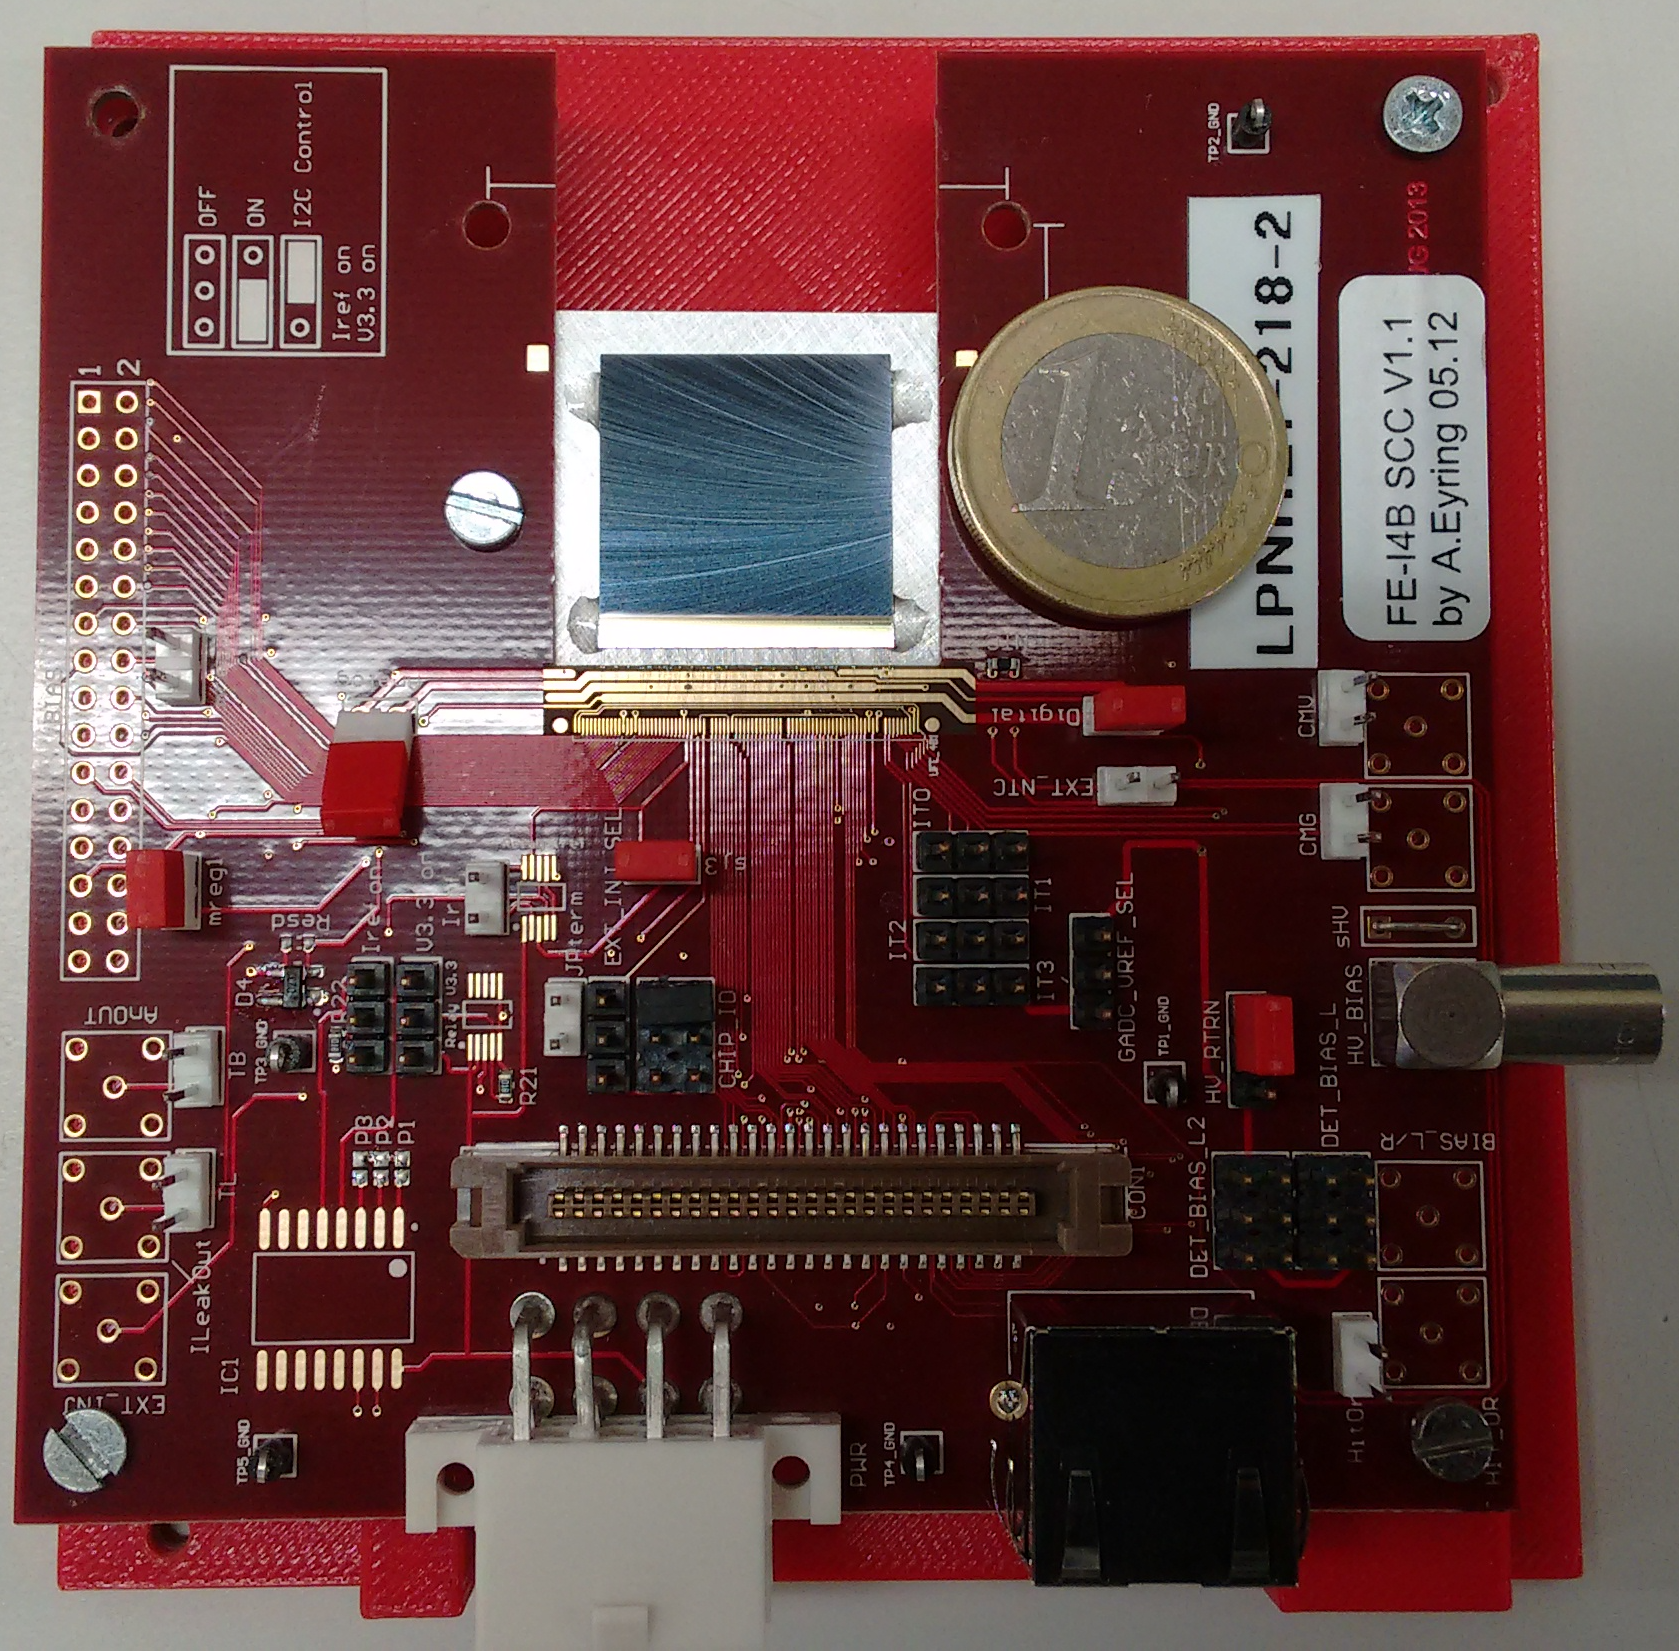
\includegraphics[width=0.35\textwidth]{scm.png}
\includegraphics[width=0.35\textwidth]{w80_irrad1.png}
\includegraphics[width=0.70\textwidth]{in_the_box.jpeg}
\caption{\label{fig:W80W30}Thin $n-on-p$ planar pixel sensor modules. (top left) Module mounted 
on a PCB card. (top right) Module inside the CERN PS irradiation area; (bottom) module inside 
the DUT cooling box at the CERN H6 beamline; W80 is the second module from the left; outside 
of the box the six planes of the ACONITE telescope~\cite{Jansen2016}.}
\end{figure}

Irradiations were carried at CERN PS using the 24~GeV/c proton beam. The irradiation was staged; 
in Table~\ref{tab:W30W80Irr} the detail of the irradiation program for the two modules tested from 
that production, $W80$ and $W30$. The two modules were taken from two different wafers, 
and had different number of GRs,  2 and 5, respectively. The final sensor assembly 
is 100~$\mum$; the 500~$\mum$  thick handle wafer was not thinned.

\begin{table}[!htpb]
\caption{\label{tab:W30W80Irr}Irradiation program for the two FE-I4 pixel modules $W80$ and $W30$.}
\centering
\begin{tabular}{cccc}
\hline 
\hline
Module name & Beam spot size & Fluence $\phi$& Cumulative fluence at  peak $\Phi$\\ 
(\# of GRs) & (FWHM - [mm$^2$]) &  [10$\times{15}$ n$_\text{eq}/\text{cm}^2$]  &  [10$\times{15}$ n$_\text{eq}/\text{cm}^2$] \\
\hline
W80 (2) & 20$\times$20 & 3 & same\\
\hline
W30 (5) & 12$\times$12 & 4 & same\\
\hline
\hline
W80 (2) & 20$\times$20 & 7 & 10 \\
\hline
W30 (5) & 20$\times$20 & 7 & 11\\
\hline
\end{tabular}
\end{table}

The modules were tested on beam after each irradiation step at CERN H6 beam line (120~GeV/c pions) and at DESY T21 beam line (4~GeV/c electrons).
 In both cases tracks were reconstructed thanks to  a EUDET-type beam telescope~\cite{Jansen2016}, 
 composed of six pixel detector planes equipped with fine-pitch MIMOSA 26 sensors~\cite{mimosa26}. 
 The DUTs where mounted inside a box that shed them from light and kept them cold 
 ($\sim$-35$^{\circ}$C).
 


\paragraph{Hit Efficiency}
Hit efficiency were tested as a function of the bias voltage for both W80 and W30 after each irradiation 
step~\cite{TrentoWS2017}. 
The results are reported in Figure~\ref{fig:HitEffW80W30} after the first irradiation step
(see Table~\ref{tab:W30W80Irr}).

\begin{figure}[!htpb]
\centering
\includegraphics[width=1.0\textwidth]{ZoomHitEffLowFl.pdf}
\caption{\label{fig:HitEffW80W30}Hit efficiency as a function of the bias voltage for W80 and W30 modules 
after the first irradiation step. The laboratory where the data were taken, the threshold and the tuning 
are indicated (HDC is a register to correct time walk effects). The red dashed line indicate the 97\% 
hit efficiency. (After~\cite{TrentoWS2017}.}
\end{figure}

The modules hit efficiency is above 97\% for bias voltages larger than 500~V. These results are good 
but somewhat below the expectations as the detectors are only 100~$\mu$m thick and the fluences 
not so elevated (3-4$\times{15}$ n$_\text{eq}/\text{cm}^2$). One possible explanation for this not 
so large hit efficiency is the threshold: 1000-1100~e were probably too high for such detectors. 

In Figure~\ref{fig:Hit_Eff_W80} the hit efficiency of W80 is reported after the second irradiation step; 
the first step is added for comparison.

\begin{figure}[!htpb]
\centering
\includegraphics[width=0.65\textwidth]{newHit_Eff_W80.pdf}
\caption{\label{fig:Hit_Eff_W80}Hit efficiency as a function of the bias voltage for the W80 module after each irradiation step.The fluence, the threshold and the tuning 
are indicated. The red dashed line indicate the 97\% 
hit efficiency.}
\end{figure}

The W80 module is 97\% efficient at a bias voltage of 600 V for a threshold of 700~e (the signal amplitude 
for a MIP in an un-irradiated module of the same thickness is about 8000~e). This result is very 
promising and it meets  the specifications for the Layer 1 of the ITk pixel detector.


The hit efficiency within the pixel cell was investigated too. In Figure~\ref{fig:NPTW80InpixelEff.pdf} 
the result for W80 after the first irradiation step. It can be seen that there are inefficient regions 
at the short sides of the pixel cell. This is consistent with the presence of permanent biasing structures 
like the $n^+$ bias dot implant and the bias rail shorting the bias dots together.

\begin{figure}[!htpb]
\centering
\includegraphics[width=1.00\textwidth]{NPTW80InpixelEff.pdf}
\caption{\label{fig:NPTW80InpixelEff.pdf} (top) Hit efficiency within a pixel of the W80 module after the first irradiation step. (bottom) The pixel cell layout is superimposed.}
\end{figure}

\paragraph{Charge Collection Efficiency}

The charge collection efficiency was studied for the W30 module after the  irradiation. The cluster charge distribution, measured in Time-over-Threshold bins of 25~ns~\cite{FEI4} was 
fitted with a Landau function convoluted with a Gaussian. In Figure~\ref{fig:IrrCCE} the comparison 
of the cluster charge distribution before and after the first irradiation step.

\begin{figure}[!htpb]
\centering
\includegraphics[width=0.75\textwidth]{IrrCCE.pdf}
\caption{\label{fig:IrrCCE}Cluster charge distribution, measured in ToT,  for the W30 module before and after the first irradiation 
step.The fluence, the threshold, the tuning, the bias voltages and the fit results are indicated.}
\end{figure}

The module was tuned always with a threshold of 1000~e and 6 ToT corresponded to 6000e. 
It can be seen that after the irradiation the most probable value (MPV) of the distribution is reduced 
by about 33\%, going from 9 to 6.

\paragraph{Comments}
Thin planar detectors are envisaged for the ITk pixel detector. The results reported here for 100~$\mu$m 
thick $n-on-p$ pixel modules are very promising since they exhibit an hit efficiency in excess of 
97\% at a bias voltage of 600~V after a fluence of 1.0$\times{16}$ n$_\text{eq}/\text{cm}^2$. The tested 
modules were just 
prototypes that used the existing FE-I4 readout chip. New thin pixels sensors prototypes, compatible 
with the RD53A chip are in preparation; thanks to new readout chip, which should have 
the possibility to get lower in threshold, it should be possible to recover full hit efficiency even at  
bias voltages lower than 600~V. 
 

\section{Edgeless Pixel Sensors}
\label{sec:edgeless}

The fractions of inactive regions are kept low by having larger pixels at the edge and in the regions between chips, and by minimising the edge region while still preventing voltage breakdown.

The 3D sensor technology inherently allows for slim edges of 15-150~$\mu$m~\cite{1748-0221-10-03-C03031}.
\section{Summary and Outlook}
\label{sec:itksummary}

